\begin{savequote}[8cm]
Energy can neither be created nor destroyed \\
Matter can neither be created nor destroyed \\
Every atom in my body goes back to the Big Bang \\
So rap is no big thang, I was created in the void
  \qauthor{---  Grip Grand, \textit{Conservation of Matter}}
\end{savequote}

\chapter{\label{ch:6-defects}H-centre defects}

\section{Introduction}

Up until this chapter we have considered a lattice with perfect translational symmetry, and no missing or extra atoms. However at finite temperature a crystalline material always contains point defects, as the cost in lattice energy is balanced by the increase in configurational entropy.
In this chapter the iodine interstitial defect is predicted to form a split-interstitial defect with self-trapped hole ($\mathrm{I}_\mathrm{i}^-+\mathrm{I}_\mathrm{i}^-+\mathrm{h}^+ \rightarrow \mathrm{I}_\mathrm{2}^-$). The vibrational properties of the defect are studied to i) confirm the validity of the 1D configurational coordinate approach and ii) predict the electron capture coefficient at this defect site.

As outlined briefly in Section \ref{recombination} we are often interested in semiconductor defects that form electronic states in the bandgap, as these can provide sites for non-radiative processes such as minority carrier trapping and electron-hole recombination, both of which limit the photovoltaic efficiency of solar cell absorber materials. Marshall Stoneham coined the term ``killer centre'' for defects with fast non-radiative transitions and lists the defect types that may act as performance killers. Two of four in the list relate to the vibrational properties of the defect lattice:

\begin{displayquote}
``2. Defects with favorable vibrational properties, that is, with large-amplitude modes promoting the transitions, and large-energy modes to take up the electronic energy.
3. Defects with very strong coupling to lattice distortions such as certain dislocations and some vacancy centers.''
\end{displayquote}

However historically there has been increased research emphasis on the electronic properties of ``killer defects'', as the calculations required to predict the vibrational properties of imperfect crystals from first principles are computationally demanding.
With recent advances in first principles modelling \cite{Alkauskas2014}%also sunghyun's paper an dalkauskas review 
and the growth in available computing power\cite{}
it is now possible to calculate from first principles the coupling strength between the electron and phonon sub-systems and predict the rate of carrier capture and recombination for systems of interest. 
This methodology has been recently applied to \ce{CZTS} where it has been found that the sulfur vacancy provides a site for fast non-radiative recombination.

Hybrid halide perovskite materials are classed in the literature as `defect tolerant' materials with low concentration of killer defects. This is for two reasons. 
Firstly, good device performance can be achieved using a low-temperature solution processing method which is expected to form a thin film with a high concentration of defects. 
%For example, the $V_\mathrm{oc}$ deficit for solution processed hybrid halide perovskite materials can be as low as \SI{0.5}{\volts}, compared to 
%http://www.nature.com/articles/srep06071
Secondly, theoretical calculations show that Schottky and Frenkel point defects form at high concentrations, but that they form electronic states either in have shallow electronic states states ($< \mathrm{kT}$ from the bandgap) which are unlikely to contribute to non-radiative recombination.
%Self-Regulation Mechanism for Charged Point Defects in Hybrid Halide Perovskites** Aron Walsh,* 
%  (http://pubs.acs.org/doi/ipdf/10.1021/jz500370k)
Amongst the native non-stochiometric defects in MAPI the iodine interstitial is predicted to be the only stable and active trap species.
%cite de angelis
% Several studies42,43 have taken advantage of absorption and emission reciprocity relationships in complete solar cells to show that the predominant contribution to the deficit in VOC from its ideal value under solar illumination is a low EQEEL value. This indicates that most carriers recombine non-radiatively. These relationships have been recently explored in mixed-cation, mixed-halide perovskites, concluding that the EQEEL is limited by SRH recombination in devices with state-of-the-art power conversion efficiency44. % https://www.nature.com/articles/nenergy2016149



The halide sub-lattice is also associated with ionic migration, with iodine ions being the dominant mobile species in MAPI.%The nature of ion conduction in methylammonium lead iodide: a multimethod approach
Experimental evidence points to a coupling between the electronic and ionic states, and various models exist which link trapping at the iodine ion with phase segregation and hysterisis in hybrid halide perovskites.
As a result, there has been recent research interest in the point defect properties of halide perovskites, and in the properties of the iodine interstitial in particular.
Point defects in hybrid halide perovskites are a challenge to model from first principles. Due to the organic cation the structure is low symmetry and there are multiple inequivalent iodine sites. The atomic lattice is soft and distorts easily, often requiring hundreds of ionic steps to achieve force convergence. 
Previous calculations in the literature demonstrate that the defect formation energies are sensitive to the level of theory used; hybrid functionals with spin-orbit coupling predict electrically active charge states of the iodine interstitial that are not found at lower levels of theory.
%mao hua du
Capacitive techniques such as Deep Level Transient Spectroscopy (DLTS) and Thermal Admittance Spectroscopy (TAS) have been used to identify defect concentrations and trap levels in the halide perovskites.
Defects have been observed with energies at SI{0.17}{\electronvolt}, SI{0.20}{\electronvolt} and SI{0.17}{\electronvolt}, SI{0.35}{\electronvolt} above valence band edge using DLTS and TAS respectively.
%https://aip.scitation.org/doi/10.1063/1.4995970
However capacitive features associated with the mobile ionic species, rather than electronic defect dynamics, can `present spectra with overlapping or even ``fake'' peaks', and it has been suggested charactiersiations with bias and light perturbations should be used to confirm the results from DLTS and TAS.
%https://pubs.acs.org/doi/abs/10.1021/acs.jpclett.9b00601

% http://pubs.acs.org/doi/abs/10.1021/acs.jpclett.5b00953 " TSC study: a peak at around T = 191 K is assigned to trap states with activation energies of around 500 meV but with a rather low concentration of 1 × 1021 m–3."

Published defect formation energies predict that the neutral iodine interstitial is metastable at all fermi levels across the bandgap.
However charge trapping at defect sites can result in the formation of metastable defects.
Meggiolaro et al. use a configuration coordinate diagram to outline the expected charge trapping processes at the iodine interstitial. 
The configuration coordinate is a collective phonon mode describing the displacement between the relevant charge states is considered and reduces the vibrational problem to one dimension.
Their model predicts that electron (hole) trapping at positively (negatively) charged defect states will result in the formation of a metastable neutral charge state, and that radiative electron trapping at the neutral defect will compete with non-radiative electron trapping.
However the rate of electron capture is not calculated, and the motion of the defect species around lattice equilibrium positions is assumed to be harmonic.


In this chapter the neutral iodine interstitial is considered. This defect is predicted to form a split-interstitial defect with self-trapped hole ($\mathrm{I}_\mathrm{i}^-+\mathrm{I}_\mathrm{i}^-+\mathrm{h}^+ \rightarrow \mathrm{I}_\mathrm{2}^-$). The hole induces the formation of a bond between two halide ions, producing an open-shell molecular dimer called a H-centre (Figure \ref{Hcentre_schematic}). The formation of a H-centre is a well-established process, and has been studied in metal halide crystals since the 1950s.
% H-center defect castner and kanzig.
The electron-phonon coupling matrix element is calculated and combined with anhamornic potential energy surfaces to give a rate for non-radiative electron capture at the H-centre (neutral) defect. In addition, all phonon modes of the defective supercell are analysed to validate the one dimensional configuration coordinate model.

%De Angelis work suggests radiative pathway between the neutral and negative charge state, we find a non-radiative pathway.
% we give carrier capture rate

\begin{figure}[h!]
\centering
  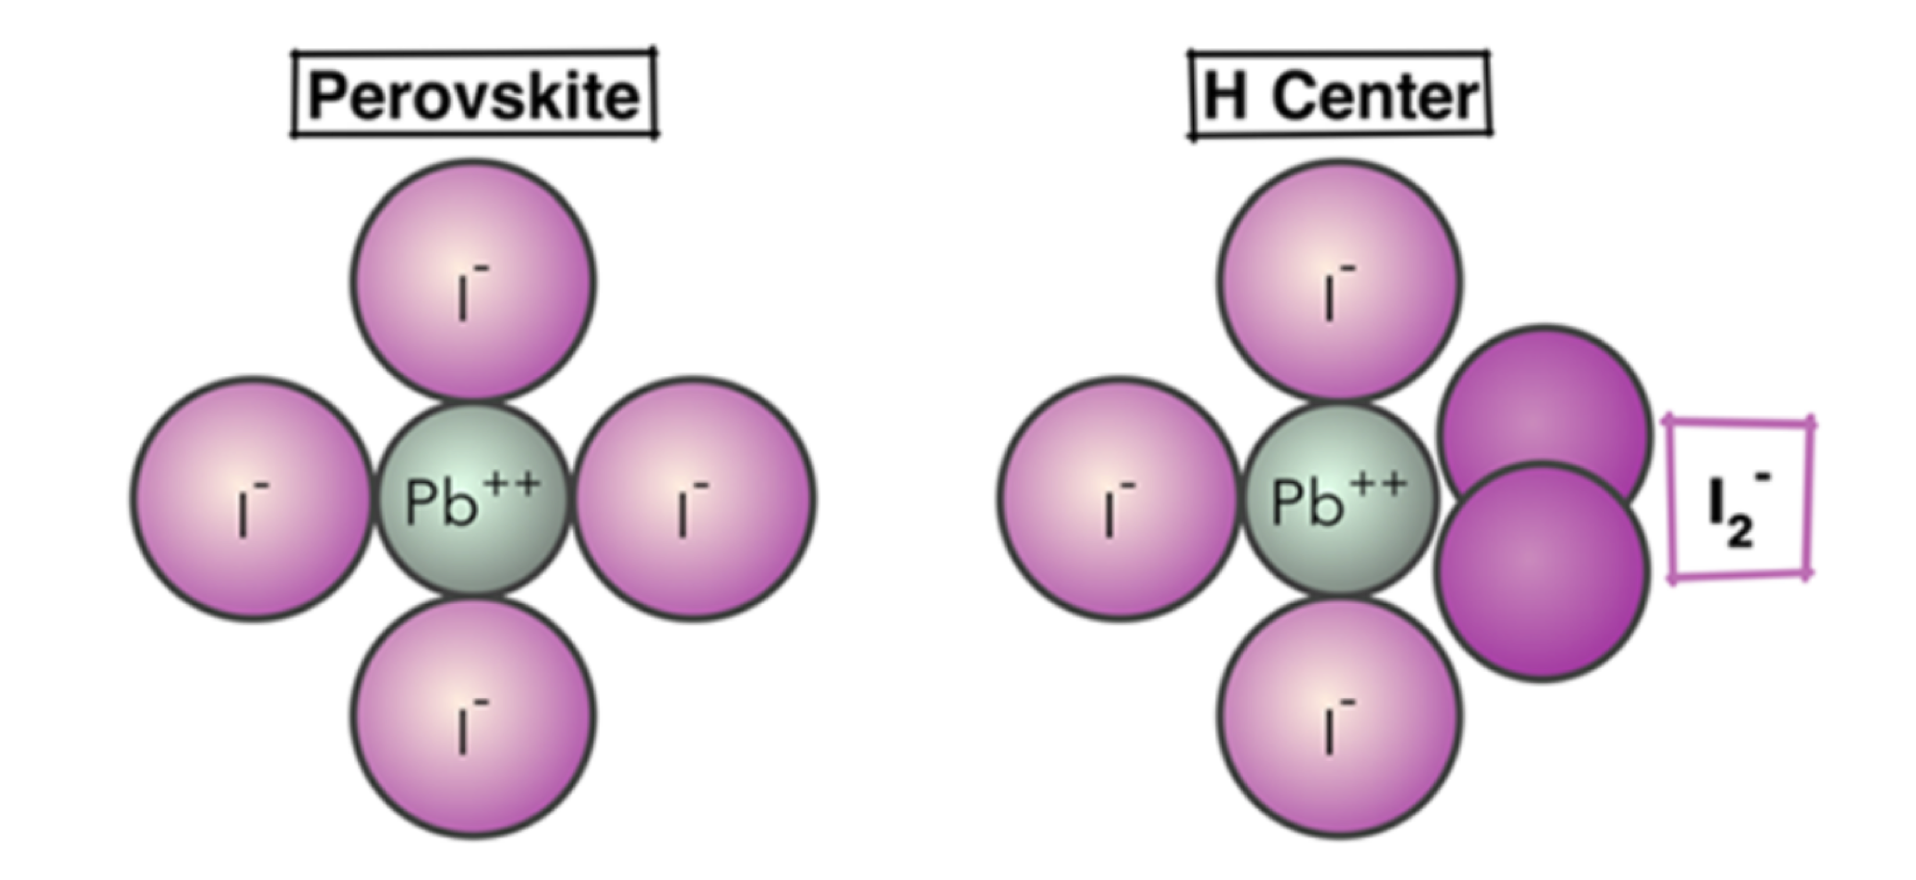
\includegraphics[width=0.7\columnwidth]{figures/ch6/Hcentre_schematic.png}
  \caption[Lattice geometry of pristine perovskite and perovskite with H-centre defect]{ Change in local equatorial environment around Pb in a lead halide perovskite upon formation of a H-center defect. The H-center the dimer is formed from a lattice iodide and interstitial iodide. The I−I interatomic spacing of ca. \SI{4.5}{\angstrom} in the perfect lattice decreases to a bond length of \SI{3.3}{\angstrom} upon dimer formation.Figure adapted with permission from an original prepared by Aron Walsh.}
\label{Hcentre_schematic}
\end{figure}


\section{Methods}

\subsection{Defect formation energies}
% ionic relaxation:PREC= NORMA LREAL = AutoEDIFF = 1.0e-05EDIFFG = -0.01ENCUT = 550ISMEAR = 0SIGMA = 0.1ISPIN = 2 (spin-polarised)
% The interstitial is placed in a 192-atom supercell, which is built from the 2\sqrt2x2\sqrt2x2 expansion of the 12-atom cubic cell, using the transformation matrix [2 -2 0 // 2 2 0 // 0 0 2]
%Ionic relaxation at HSE06 confirms that there is very little distortion from PBEsol relaxed structure.
% Perfect structure confirmed stable from a phonon calculation.

% Using the HSE06 hybrid functional with spin-orbit coupling, and a 2x2x2 sampling of the electronic brillouin zone (gamma centred).PREC= NORMALREAL = AutoLCHARG = .TRUE.EDIFF = 1.0e-06ENCUT = 550SIGMA = 0.1. bandgap is correct with correct alpha.

% Using Daint. Importance of ROPT. Importance of alpha parameter

% convergence studies with number of atoms



\subsection{Lattice dynamics}

\subsection{Carrier capture rates}

% @sunghyun will have to correct me if I'm wrong but my understanding is that the waveunctions generated by vasp are not orthogonal so its not valid to calculate the overlap using the dot product. Pawpyseed can be used to orthogonalise the wavefunctions and then dot products can be done
% Yes, a WAVECAR file contains only the plane-wave coefficients for the smooth pseudo wave function and we also need the core part to do anything with the all-electron wave function.
% scaling factor not needed as neutral
% input the parameters (like degeneracy) from the input files
\section{Results} \label{ch:6-results}

\subsection{Defect geometry}
%include diagram of relaxation workflow with energies marked. Highlight why nice doing from cubic starting structure.
% consider in all charge states due to where the fermi nergy is.
% schematic of lowest energy structures found: -/neutral/positive.
% description of each - in-plne vs out of plane
% how this compares to literature
%  bonding lengths - is this closer to optimal? lattice distorts so can get close?
% include significance of large distortion: in plane to out of plane
% include displacement vectors
% talk about breaking symmetry. Why we chose cubic: not decided already how broken.
% need to manually break symmetry - testing for lower energy.
% different depending on starting point: pockets of minima

\subsection{Charge localisation}
%plot spin density
% including TDDFT
% Following the“molecule in crystal”approach7with dielectricembedding, we computed the optically excited states of the Cl2−,Br2−, and I2−defect centers as a function of bond lengths usingtime-dependent DFT (seeFigure 2) including relativistic effect
% However, certain point defects can act as color centers,with charge-conserving optically excited states. For example, thecolor (F) centers consisting of an electron trapped at a vacantlattice site in alkali halides, or self-trapped holes in heteropolarcrystals that are termed V-centers.
%Previous section look at large polaron, in this one a small polaron is considered.

\subsection{Defect formation energies}

% formula
% defect corections very small: do sxdefectalign output in appendix
% using previously published dielectric for ionic?
% tilting correction results: 
    %We expect the tilting correction to scale linearly with supercell size
    %See work published in Ruoxi's thesis
    %270/37 = 7.5 ~ 8 which is to be expected as supercell is 8* bigger
    %We expect reduction of 2*37meV for 192 supercell = 0.074eV
     % Schematic of what is happening Although small, important as exponential term.
% negative U behaviour
% two electron nature: no trapping

\subsection{Vibrational properties}
% including IPR
% Emphasise that the agreement between IPR and configuration coordinate shows that the approximation of a 1D PES is great in this instance.
%upload on Youtube
% include Julia phonons work! distortion projected 

\subsection{Configuration Coordinate diagram}

% for lovely discussion see Alkauskas:
% https://www.osti.gov/pages/servlets/purl/1471061
%"It might be surprising that this one-dimensional approximation to what is
%essentially a multi-dimensional problem (where the dimensionality is 3N, N being the number of atoms in the system) is
%sufficient. The beauty of 1D cc diagrams is that often they are
%sufficient.51 As discussed in the Appendix, this is particularly the
%case for defects with strong electron–phonon coupling. In certain
%cases, the validity of this approximation can be demonstrated rigorously; we discuss one such example in the Appendix."

% Need to make CC diagram. 
% All the CC diagrams should be referenced to zero.
% use linear interpolation
% interpert CC
% CC diagram with schrodinger solution superimposed.
% problem with the adiabatic approach and falling to the local minima
% talk ahout the difference between the photochemistry and equilibrium thermodynamics
% calculate the harmonic PES to show why the anharmonic is important


\subsection{carrier capture rate}

% how carrier capture is calculated - alkauskas.
% importance of suitable starting state and state to capture into
% then the eigenvalues with distortion and overlap/gradient of overalpt....
% emphasise that the carrier capture rate (EP coupling) is lower than expected - reason for good behaviour.

% guidance for synthesis?

% confirmed that coupling away from band edge is reduced (0.002 CBM and 0.0099 VBM)

\textbf{Summary}
% Future work around the interaction between electronic and ionic states.
%  Themolecular iodide defects discussed here are not necessarily staticcarrier traps, because the halides that form the corner-sharingperovskite framework support reasonable rates of ion transport.Room-temperature diffusion is expected for the V-center, whichcould proceed in a pathway akin to vacancy-mediated diffusion.
% Transport of the H-center would require an interstitialcymechanism, which has also been predicted to be low energy inhalide perovskites.12The slow motion of trapped holes wouldadd a further layer to the complexity of the temporal response ofperovskite solar cells to light soaking and bias voltages (alsoevident in quantum dot photovoltaics13). Given the polyanionnature of iodine (e.g., charged I2up to I16complexes) and theflexibility of the perovskite structure, the formation of largercharged molecular aggregates is also possible for the iodideperovskites. Such polyanion inclusions in a crystal would beredox active and could facilitate additional electron or holetrapping, which is a fertile line of research for future studie
% interstitcalicy - sam stranks paper
% open questions around interface and recomgination" JS Park, It has been reported that grain boundaries do not act as charge recombination centres (Edri nanoletters 2014,14,1000-1004)
%  This poses a challenge for computational modelling as processes over a range of time and length scales are coupled together. 
% interested in minority carrier capture, but roughly equal holes and electronis in perovskite??? so both of interest. holes are slightly more bountiful, so wrt limiting current collection, it is hole capture.

\textbf{Data access statement}
% I need to publish my structures!
% displacement vectors
% carrier capture code
%pawpyseed
%phonopy
% modemap

\textbf{Acknowledgements}

Calculations were performed on the SiSu supercomputer at the IT Center for Science (CSC), Finland, via the Partnership for Advanced Computing in Europe (PRACE) project no. 13DECI0317/IsoSwitch.
% Need to include TDDFT at start thesis